\documentclass[11pt]{article}
\usepackage{amssymb}
\usepackage[english]{babel}
\usepackage{fullpage}
\usepackage{graphicx}
\usepackage{pythonhighlight}
\usepackage{listings}


\def\titre{}
\def\auteur{}
\def\courriel{}
\makeatletter

\title{}

\author{}

\date{}

\begin{document}
\maketitle
\section{Flask deployment}

\paragraph{Deployment on LINUX (EC2 instances)}\mbox{}\\
On each instance, the flask app is deployed when the instance is in a running state. The python application is created in the directory home/ubuntu/flask-server after installing a python virtual environment and flask. The application runs on 0.0.0.0 at port 80. The bash script to be executed in each instance is contained in a python file (app\_cluster1.py and app\_cluster2.py). For machines in the cluster 1, the app will route the requests to the URL /cluster1, and for machines in cluster 2, the app will route the requests to the URL /cluster2. A health check can be performed by sending a request without a path, and the response returned will be
\begin{lstlisting}[language=C]
Healthy!
\end{lstlisting}
If the URL path contains either /cluster1 or /cluster2, the resonse returned will be
\begin{lstlisting}[language=C]
Instance {AWS_INSTANCE_ID} is responding now!
\end{lstlisting}
Where AWS\_INSTANCE\_ID is the ID of the instance that responded to the request.

\section{Infrastructure setup}

\paragraph{Instances}\mbox{}\\
The instances created will be five M4.large instances (two 2.4 GHz Intel Xeon E5-2676 vCPUs, 8 GiB memory, moderate network performance and 450 Mbps) (Amazon Web Services, n.d.) and five T2.large instances (two Intel vCPUs, 8 GiB of memory and low to moderate network performance)  (Amazon Web Services, n.d.). However, due to account restrictions, we can only deploy a total of nine instances, so the second group will only have four. Each instance will allow SSH, HTTP and HTTPS traffic from 0.0.0.0/0, meaning the whole internet. The operating system is ubuntu and the image used is ami-08c40ec9ead489470. The availability zone will be us-east-1. Flask will be deployed on each instance at IP address 0.0.0.0 port 80. The storage is EBS-Only for both instances.  (Amazon Web Services, n.d.)

\begin{table}[h!]
    \caption{Specs of M4.large and T2.large}
    \label{tab:table1}
    \begin{tabular}{|l|c|c|c|c|r|}
        \hline
        \textbf{Type} & \textbf{vCPU} & \textbf{Memory (GiB)} & \textbf{EBS Bandwidth (Mbps)} & \textbf{Network performance}\\
        M4.large & 2 & 8 &450 &Moderate\\
        T2.large & 2 & 8 &- &Low to Moderate\\
        \hline
    \end{tabular}
\end{table}

\paragraph{Target groups:}\mbox{}\\
The first target group will include all five M4.large instances, while the second one will be four T2.large instances. The targets will receive traffic on port 80. IPv4 will be used with the HTTP protocol.

\paragraph{Elastic load balancer:}\mbox{}\\
The elastic load balancer will be an internet facing application load balancer (requests can be routed based on their contents such as the URL path). IPv4 is used. Its security group allows it to send and receive traffic from anywhere on the internet (TCP to and from 0.0.0.0/0). Two subnet IDs are specified (us-east-1a and us-east-1b).

\paragraph{Listener}\mbox{}\\
The listener listens on port 80 and will send requests to one of the two target groups that are attached to it. The protocol is HTTP, and both target groups are given equal weight. The URL path for the first target group is /cluster1 and the URL path for the second target group is /cluster2. The paths are specified in the value

\begin{python}[h!]
    Conditions=[
        {
            'Field': 'path-pattern',
            'PathPatternConfig': {
                'Values': [
                    path
                ]
            },
        },
    ],
\end{python}

\paragraph{Auto Scaling}\mbox{}\\
Each target group will be in a separate auto scaling group. The autoscaling groups will be in different subnets (us-east-1a and us-east-1b). Since we can only have 9 instances, each target group will have minimum of four instances and a maximum of five instances. The launch template contains the necessary data to create the instances, including the security groups, the instance type and the user data that will be executed when the instances are running.

\paragraph{Deployment}
\begin{enumerate}
    \item Two launch templates are created with the necessary info to launch instances (instance type, user data, key name and security groups)
    \item 2 target groups are created (target-group-1 and target-group-2)
    \item A security group for the elastic load balancer is created
    \item The load balancer lab1-load-balancer is created with the attached security group
    \item A listener is created and the two target groups are attached to the listener; the two target groups have equal weight. The protocol used is HTTP.
    \item Rules are created for routing the traffic with path /cluster1 to target-group-1 and /cluster2 to target-group-2. target-group-1 has a higher priority than target-group-2
    \item The auto scaling groups group1 and group2 are created with the previously created templates. They are in different subnets.
    \item The program waits for the instances to deploy flask.
\end{enumerate}
The diagram of the setup is as follows:\\

% \begin{figure}
%     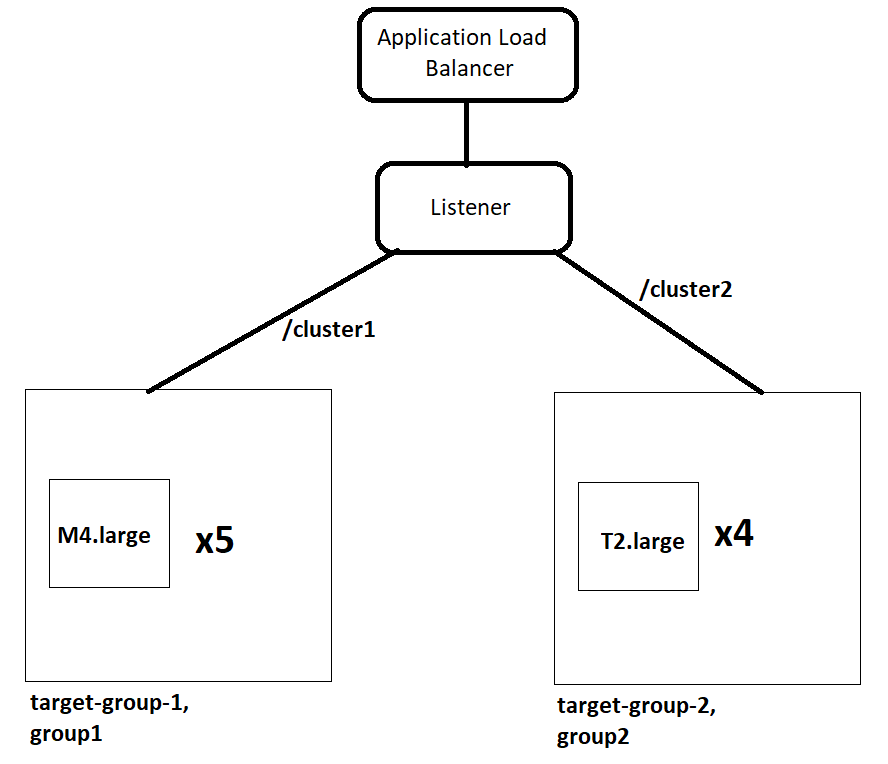
\includegraphics[width=0.5\linewidth]{cluster.png}
%     \caption{Application load balancer with 2 clusters and a forward listener}
%     \label{fig:setup}
% \end{figure}
\begin{center}
    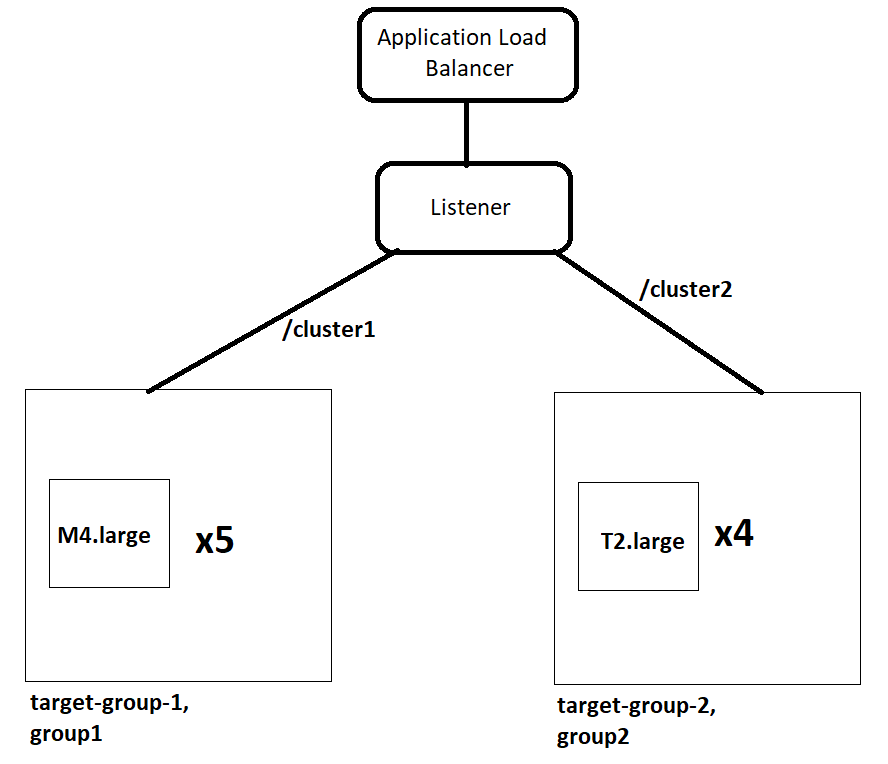
\includegraphics[scale=0.5]{cluster.png}\\
    Figure 1. Application load balancer with 2 clusters and a forward listener  
\end{center}

\section{References}
Amazon Web Services. (n.d.). {\it Amazon EC2 Instance Types}. Amazon Web Services. Retrieved October 17, 2022, from https://aws.amazon.com/ec2/instance-types/ 

\end{document}
